\section{Introducci\'on}

En esta sección se implementarán heuristicas de busqueda local para tratar de resolver el problema de $k-PMP$, intentando con diferentes metodos para alcanzar una solución y diferentes vecindades.

Para ello, partiendo de una solución generada al azar, se intentará a travez de sucesivas iteraciones analizar sierta vecindad para intentar mejorar la solución existente y aproximarse mas a una 'buena' solución en un tiempo aceptalble. 

Por lo tanto debemos tener en cuenta de no hacer las vecindades ni muy grandes, ya que esto puede llevar a una perdida de performance, ni muy pequeñas, ya que esto puede llevar a que el algoritmo explore solo una pequeña cantidad de soluciones y devuelva una solución muy alejada del optimo.

Como primera idea para una vecindad tomaremos cada nodo del grafo, vemos cuanto peso agrega en la suma intraconjunto en que se encuentra, lo quitaremos de este conjunto e intentamos meterlo en todos los demas, viendo si en alguno logra minimizar esta suma. En caso afirmativo, lo sacamos de su antiguo conjunto y lo ponemos en el nuevo. Realizamos esto hasta que deja de ser posible mejorar la solución y en este punto la devolvemos.

Esta heuristica, como se verá en el apartado de testing, devuelve resultados vastante aproximados, al compararlo con la solución exacta y con las otras heuristicas.

Otra vecindad que plantearemos será buscar el nodo que mas peso esta generando en la suma intrapartición, quitarlo de la partición donde se encuentra y agregarlo a alguna otra.

Finalmente se implementará una tercera busqueda local que quite dos nodos que estan en una misma partición e intente buscar alguna otra donde los mismos sumen un menor peso intrapartición.

Los algoritmos escritos de manera mas formal serán así:

\begin{algorithm}
  	\begin{algorithmic}[1]\parskip=1mm
		 \caption{ Busqueda1(SoluciónInicial) }
		 	\STATE{Guardo SoluciónInicial en SolucionPrevia}
	 		\STATE{Mientras en el paso anterior se haya mejorado SolucionPrevia} 
				\STATE{\quad Tomo un nodo $i$ de $1$ a $n$ del grafo}
		 		\STATE{\quad Miro que peso agrega el nodo $i$ en el conjunto asignado por SolucionPrevia}
		 		\STATE{\quad Miro que peso agrega el nodo $i$ quitandolo del conjunto asignado y poniendolo en los demas}
				\STATE{\quad \quad Si En algun conjunto $M$ obtengo un peso menor, modifico SolucionPrevia y asigno $i$ al conjunto $M$}   
				\STATE{\quad \quad Itero}
	\end{algorithmic}
\end{algorithm}

\begin{algorithm}
  	\begin{algorithmic}[1]\parskip=1mm
		 \caption{ Busqueda2(SoluciónInicial) }
			\STATE{Guardo SoluciónInicial en SolucionPrevia}
	 		\STATE{Mientras en el paso anterior se haya mejorado SolucionPrevia}
			\STATE{Asigno $j = 1$}
				\STATE{\quad Tomo el j-esimo nodo mas pesado de la SolucionPrevia, al que llamo $i$}
		 		\STATE{\quad Miro que peso agrega el nodo $i$ en el conjunto asignado por SolucionPrevia}
		 		\STATE{\quad Miro que peso agrega el nodo $i$ quitandolo del conjunto asignado y poniendolo en los demas}
				\STATE{\quad \quad Si En algun conjunto $M$ obtengo un peso menor}   
				\STATE{\quad \quad \quad modifico SolucionPrevia y asigno $i$ al conjunto $M$}
				\STATE{\quad \quad \quad Itero}
				\STATE{\quad \quad Si no, sumo $1$ a $j$}
				\STATE{\quad \quad Si $j == n$}
				\STATE{\quad \quad \quad Devuelvo SolucionPrevia}
				\STATE{\quad \quad Si no}
				\STATE{\quad \quad \quad Itero}
	\end{algorithmic}
\end{algorithm}

\begin{algorithm}
  	\begin{algorithmic}[1]\parskip=1mm
		 \caption{ Busqueda3(SoluciónInicial) }
		 	\STATE{Guardo SoluciónInicial en SolucionPrevia}
	 		\STATE{Mientras en el paso anterior se haya mejorado SolucionPrevia} 
				\STATE{\quad Tomo un nodo $i$ de $1$ a $n$ del grafo}
				\STATE{\quad\quad Tomo otro nodo $k$ del conjunto de $i$}
		 		\STATE{\quad\quad Miro que peso agrega el nodo $i$ y $k$ en el conjunto asignado por SolucionPrevia}
		 		\STATE{\quad\quad Miro que peso agrega el nodo $i$ y $k$ quitandolo del conjunto asignado y poniendolo en los demas}
				\STATE{\quad\quad \quad Si En algun conjunto $M$ obtengo un peso menor, modifico SolucionPrevia y asigno $i$ y $k$ al conjunto $M$}   
				\STATE{\quad\quad \quad Itero}
	\end{algorithmic}
\end{algorithm}

\section{complejidades}

Ahora aquí analizaremos las complejidades de los diferentes algoritmos. Para cada uno de ellos elegimos una implementacion con matriz de adyacencias para modelar el peso de las aristas y un vector de longitud variable para implementar los diferentes conjuntos.

Para el primero, cada paso de busqueda local tendrá una complegidad de peor caso de $O(n(n + n k + n^2))$. Ahora si $k$ es mayor a $n$ quiere decir que hay mas subconjuntos disponibles que nodos, lo que llevaría a una solución trivial donde cada nodo va en un subconjunto diferente y la solución para $k-PMP$ sería 0.
Luego podemos acotar a $k$ por $n$ con lo que se obtendría una complegidad igual a $O(n^3)$

Para el segundo algoritmo, por cada iteración del algoritmo la complegidad será $O(n^2)$ para calcular el nodo con mayor peso del grafo. $O(k n)$ para determinar si existe una mejor partición donde este nodo pueda estar y, en el caso de que exista, $O(n^2)$ para quitarlo de la partición anterior y agregarlo a la nueva. Luego, nuevamente acotando $k$ por $n$, se obtiene una complegidad para cada paso de la iteración de $O(n^2)$.

El tercer algoritmo es simplemente el primer algoritmo pero esta vez. para cada nodo ademas tomo un vecino, y realizo el mismo procedimiento que antes, esto para cada vecino, suponiendo que en el peor caso, para un nodo todos los otros nodos esten en el mismo conjunto, se tendrá que realizar el procedimiento de antes la misma cantidad de veces solo que ahora para dos nodos distintos, luego la complejidad continúa siendo $O(n^2 (n + n k + n^2))$. Acotando nuevamente $k$, obtenemos que el algoritmo es: $O(n^3)$

\section{Testing}

En esta sección comprobaremos de manera empirica las complejidades antes calculadas y luego una comparación entre las tres diferentes heuristicas.

Para ello, al ignal que para el algoritmo goloso, tomamos grafos completos con 25 a 100 nodos, y comparamos los diferentes tiempos obtenidos:

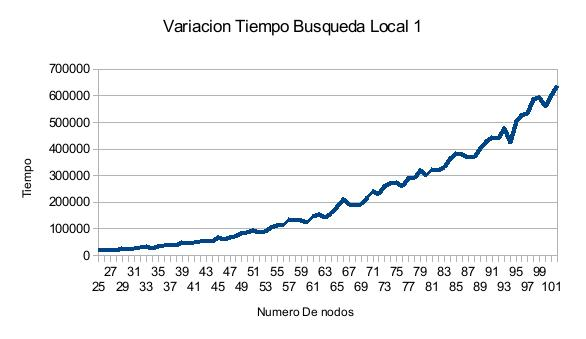
\includegraphics[scale=0.5]{Ej4/tiempo1.jpg}

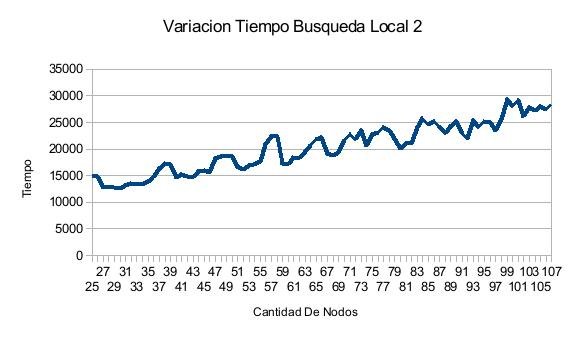
\includegraphics[scale=0.5]{Ej4/tiempo2.jpg}

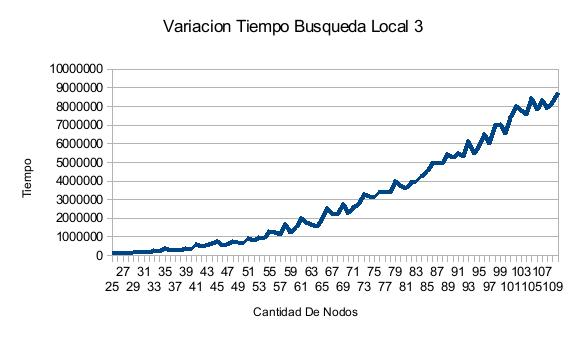
\includegraphics[scale=0.5]{Ej4/tiempo3.jpg}

Puede verse que si bien existe sierto ruido en la toma de muestras, causado muy posiblemente por el hecho de que para cada grafo, el numero de veces que es posible continuar mejorando la solución sea variable y poco controlable. Existe una tendencia muy marcada en los tres algoritmos.

Para poner mas en evidencia esto, dividiremos por las complegidades teoricas para asi hacer mas evidente este patron:

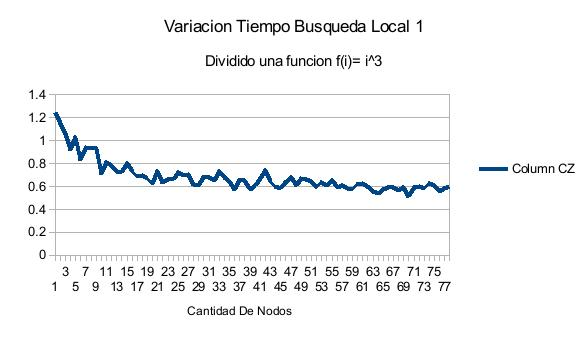
\includegraphics[scale=0.5]{Ej4/tiempo1div.jpg}

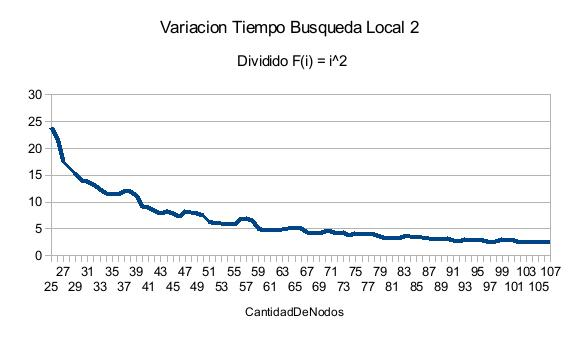
\includegraphics[scale=0.5]{Ej4/tiempo2div.jpg}

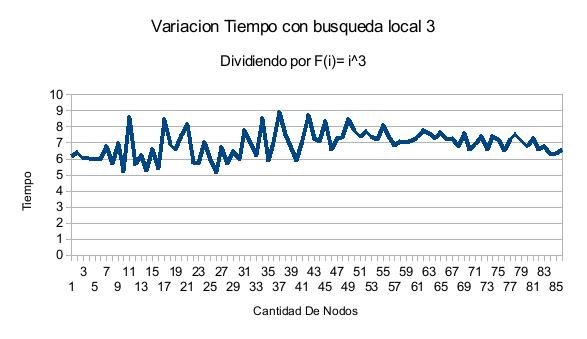
\includegraphics[scale=0.5]{Ej4/tiempo3div.jpg}

Como puede verse, en los tres casos las heruristicas son acotadas por las complegidades calculadas en el apartado anterior.

Ahora, para 100 grafos completos con un numero fijo de nodos igual a $23$, y aristas tomadas de $1$ a $100$, compararemos los resultados obtenidos con backtracking con los obtenidos por estas heuristicas.

Los resultados arrojados son los siguientes:

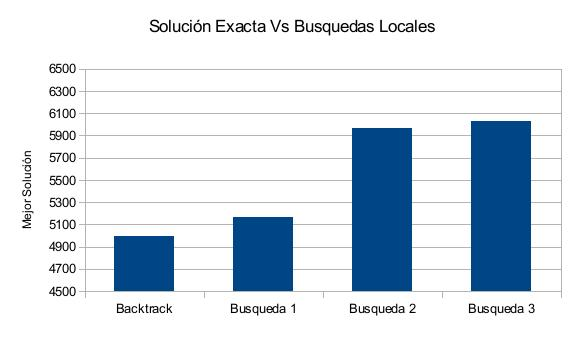
\includegraphics[scale=0.5]{Ej4/solucionestodos.jpg}

Puede verse que el que mejor aproxima a las soluciones reales es la primera busqueda local. Y no solo eso, de los 100 casos tomados, la busqueda local 1 logra encontrar la solución exacta a 13 de las instancias! mientras que las otras dos heuristicas en ninguno de los casos logran encontrar la solución exacta.

Ademas, para estas instancias se realiza a modo comparativo un promedio de los tiempos que tardan en encontrar la solución, esto es lo que se obtiene:

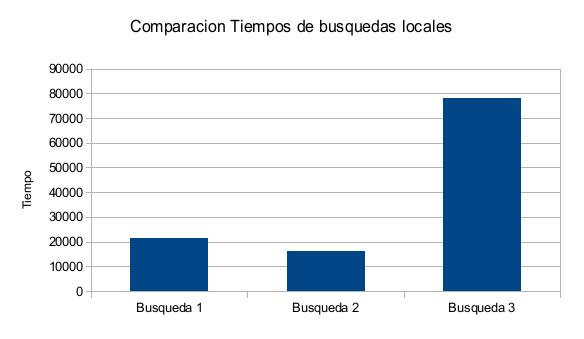
\includegraphics[scale=0.5]{Ej4/tiempotodos.jpg}

Por lo que en primera instancia, el algoritmo de busqueda local 1 es bastamente superior en todo sentido a los otros dos. Encuentra soluciones exactas, y obtiene tiempos empiricos mucho mejores que los otros dos algoritmos.